% !TEX root = ../main.tex

\chapter{Problemas Adicionales}
\label{chap:problemas_adicionales}

% ==============================================================================
% SECCIÓN 1: BÁSICOS
% ==============================================================================

\section{Problemas básicos}

\subsection*{1. Masa Nuclear, Defecto de Masa y Energía de Ligadura}

La masa de un átomo neutro $M(Z,A)$ constituido por $Z$ protones y $N = A - Z$ neutrones es siempre inferior a la suma de las masas de sus nucleones componentes libres ($Z$ átomos de hidrógeno ${}^1\text{H}$ y $N$ neutrones $n$):
\begin{equation}
M(Z,A) < Z M({}^1\text{H}) + N m_n
\end{equation}

Esta diferencia de masa se denomina \textbf{defecto de masa} ($\Delta M$) y representa la energía liberada durante la formación del estado ligado nuclear:
\begin{equation}
\Delta M(Z,A) \equiv Z M({}^1\text{H}) + N m_n - M(Z,A)
\end{equation}

La \textbf{energía de ligadura} ($B$) es la energía mínima necesaria para disgregar completamente un núcleo en sus nucleones constitutivos individuales:
\begin{equation}
B(Z,A) = \Delta M(Z,A) c^2 = \left[ Z M({}^1\text{H}) + (A - Z) m_n - M(Z,A) \right] c^2
\end{equation}

En la práctica, las masas atómicas se expresan en unidades de masa atómica ($\text{u}$), donde $1\text{ u} \equiv 1/12 \, M({}^{12}\text{C}) \approx 931.5\text{ MeV}/c^2$. La estabilidad relativa entre diferentes núcleos se mide mediante la \textbf{energía de ligadura por nucleón} ($B/A$), la cual alcanza un máximo de aproximadamente $8.7\text{ MeV/nucleón}$ en la región del hierro ($A \approx 56$).

\subsection*{2. Distribuciones de Carga, Factor de Forma y Energía Culombiana}

\subsubsection*{2.1. Factor de forma y radio cuadrático medio}
La distribución espacial de la carga nuclear $\rho(\vec{r})$ determina la desviación de la dispersión de electrones respecto a la dispersión puntual de Rutherford. El \textbf{factor de forma electromagnético} $G(q^2)$ es la transformada de Fourier de la densidad de carga:
\begin{equation}
G(q^2) = \int \rho(\vec{r}) e^{i \vec{q} \cdot \vec{r} / \hbar} d^3r
\end{equation}

Para transferencias de momento pequeñas ($q^2 \to 0$), el desarrollo en serie del factor de forma relaciona directamente su pendiente con el \textbf{radio cuadrático medio} $\langle r^2 \rangle$:
\begin{equation}
G(q^2) = 1 - \frac{1}{6\hbar^2} \langle r^2 \rangle q^2 + \mathcal{O}(q^4) \implies \langle r^2 \rangle = -6\hbar^2 \left. \frac{d G(q^2)}{d(q^2)} \right|_{q^2=0}
\end{equation}

\subsubsection*{2.2. Energía de repulsión de Coulomb}
La repulsión electrostática entre los protones genera una energía potencial de Coulomb $U_c$ que reduce la ligadura del núcleo ($B = B_{\text{fuerte}} - U_c$). Para una carga total $Q = Z e$ repartida en una esfera de radio $R$:
\begin{itemize}
    \item \textbf{Distribución volumétrica homogénea:}
    \begin{equation}
    U_c(\text{vol}) = \frac{3}{5} \frac{1}{4\pi\varepsilon_0} \frac{Z(Z-1) e^2}{R}
    \end{equation}
    \item \textbf{Distribución superficial pura:}
    \begin{equation}
    U_c(\text{sup}) = \frac{1}{2} \frac{1}{4\pi\varepsilon_0} \frac{Z(Z-1) e^2}{R}
    \end{equation}
\end{itemize}

El cociente entre ambas configuraciones es constante:
\begin{equation}
\frac{U_c(\text{vol})}{U_c(\text{sup})} = \frac{3/5}{1/2} = \frac{6}{5} = 1.2
\end{equation}

En los \textbf{isóbaros espejo} ($Z_1 = Z, N_1 = Z-1$ frente a $Z_2 = Z-1, N_2 = Z$), la interacción fuerte es idéntica ($V_{pp} \approx V_{nn}$). Por ello, la diferencia entre sus energías de ligadura permite determinar experimentalmente el radio nuclear común $R$:
\begin{equation}
\Delta B = B(Z-1, A) - B(Z, A) = U_c(Z) - U_c(Z-1) = \frac{3}{5} \frac{e^2}{4\pi\varepsilon_0 R} \left[ Z(Z-1) - (Z-1)(Z-2) \right]
\end{equation}

\subsection*{3. Valor $Q$ de una Reacción Nuclear y Desintegraciones}

Consideramos una reacción nuclear general expresada como $a + A \longrightarrow b + B$. La conservación de la energía relativista en el sistema del laboratorio (donde el blanco $A$ está en reposo) establece:
\begin{equation}
m_a c^2 + K_a + m_A c^2 = m_b c^2 + K_b + m_B c^2 + K_B
\end{equation}

Se define el \textbf{valor $Q$ de la reacción} como la diferencia entre las energías en reposo iniciales y finales, equivalente al balance cinético:
\begin{equation}
Q \equiv \left[ (m_a + m_A) - (m_b + m_B) \right] c^2 = K_b + K_B - K_a
\end{equation}

Si las masas se expresan en unidades de masa atómica ($\text{u}$), el cálculo directo de $Q$ resulta:
\begin{equation}
Q = \Delta m \times 931.5\text{ MeV/u}, \quad \text{con } \Delta m = (m_a + m_A) - (m_b + m_B)
\end{equation}

\subsubsection*{Clasificación cinemática:}
\begin{itemize}
    \item \textbf{Reacción Exoérgica ($Q > 0$):} Hay una conversión neta de masa en energía cinética. Puede ocurrir espontáneamente a cualquier energía de los reactivos.
    \item \textbf{Reacción Endoérgica ($Q < 0$):} Requiere absorber energía cinética externa. La partícula proyectil debe superar la \textit{energía umbral} ($K_{\text{umb}} = |Q| (1 + m_a/m_A)$) para que la reacción sea cinemáticamente posible.
\end{itemize}

\subsubsection*{Desintegraciones radiactivas:}
Para un núcleo inestable que decae de forma espontánea ($A \longrightarrow B + c$):
\begin{equation}
Q = (M_A - M_B - m_c) c^2
\end{equation}
\begin{itemize}
    \item La condición necesaria y suficiente para que la desintegración sea espontáneamente viable es $Q > 0$.
    \item En la desintegración $\beta^-$ ($n \to p + e^- + \bar{\nu}_e$), el valor $Q_{\beta^-}$ corresponde a la energía cinética máxima $T_{e,\text{máx}}$ que puede transportar el electrón.
\end{itemize}

\newpage

\begin{problema}[Reacción nuclear ${}^{14}\text{N}(n,p){}^{14}\text{C}$ y Valor $Q$]
Dada la reacción nuclear ${}^{14}\text{N}(n,p)?$:
\begin{enumerate}[label=\alph*)]
    \item Complete la reacción identificando el núcleo resultante.
    \item Calcule el valor $Q$ de la reacción en $\text{MeV}$ e indique si el proceso es exoérgico o endoérgico.
\end{enumerate}

\textbf{Datos de masas atómicas:} $M({}^{14}\text{N}) = 14.003074\text{ u}$, $m_n = 1.008665\text{ u}$, $M({}^1\text{H}) = 1.007825\text{ u}$, $M({}^{14}\text{C}) = 14.003242\text{ u}$, $1\text{ u} \cdot c^2 = 931.5\text{ MeV}$.

\tcblower

\subsubsection*{a) Completar la reacción nuclear}

Representamos la reacción nuclear con la notación genérica $a + A \longrightarrow b + X$:
\begin{equation}
{}_0^1 n + {}_7^{14}\text{N} \longrightarrow {}_1^1 p + {}_Z^A X
\end{equation}

\begin{center}
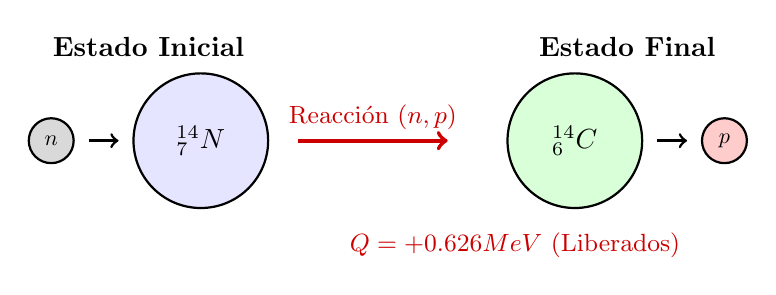
\begin{tikzpicture}[scale=0.95]
  % Estado Inicial
  \draw[thick, fill=blue!10] (-3.5,0) circle (0.9) node[black] {${}_7^{14}\text{N}$};
  \draw[thick, fill=gray!30] (-5.5,0) circle (0.3) node[black, scale=0.8] {$n$};
  \draw[->, line width=1pt] (-5.0,0) -- (-4.6,0);
  \node[above] at (-4.2, 1.0) {\textbf{Estado Inicial}};

  % Flecha Reacción
  \draw[->, line width=1.5pt, red!80!black] (-2.2,0) -- (-0.2,0) node[midway, above] {\small Reacción $(n,p)$};

  % Estado Final
  \draw[thick, fill=green!15] (1.5,0) circle (0.9) node[black] {${}_6^{14}\text{C}$};
  \draw[thick, fill=red!20] (3.5,0) circle (0.3) node[black, scale=0.8] {$p$};
  \draw[->, line width=1pt] (2.6,0) -- (3.0,0);
  \node[above] at (2.2, 1.0) {\textbf{Estado Final}};
  \node[red!80!black] at (0.7, -1.4) {\small $Q = +0.626\text{ MeV}$ (Liberados)};
\end{tikzpicture}
\end{center}

Aplicando las leyes de conservación del número atómico ($Z$) y del número másico ($A$):
\begin{itemize}
    \item \textbf{Conservación de la carga ($Z$):} $0 + 7 = 1 + Z \implies Z = 6$ (Carbono, $\text{C}$).
    \item \textbf{Conservación del número de nucleones ($A$):} $1 + 14 = 1 + A \implies A = 14$.
\end{itemize}

Por consiguiente, el núcleo producido es Carbono-14 (${}^{14}\text{C}$) y la ecuación completa de la reacción es:
\begin{equation}
{}^{14}\text{N}(n,p){}^{14}\text{C} \quad \Longleftrightarrow \quad {}_0^1 n + {}_7^{14}\text{N} \longrightarrow {}_1^1 p + {}_6^{14}\text{C}
\end{equation}

\subsubsection*{b) Cálculo del valor $Q$ de la reacción}

El valor $Q$ se define como el balance entre la masa total inicial de los reactivos y la masa total final de los productos:
\begin{equation}
Q = \left[ (m_n + M({}^{14}\text{N})) - (M({}^1\text{H}) + M({}^{14}\text{C})) \right] c^2
\end{equation}

Calculamos en primer lugar el defecto de masa ($\Delta m$):
\begin{align}
\Delta m &= (1.008665\text{ u} + 14.003074\text{ u}) - (1.007825\text{ u} + 14.003242\text{ u}) \nonumber \\
&= 15.011739\text{ u} - 15.011067\text{ u} = 0.000672\text{ u}
\end{align}

Convertimos el defecto de masa a energía utilizando el factor de equivalencia $931.5\text{ MeV/u}$:
\begin{equation}
Q = 0.000672\text{ u} \times 931.5\text{ MeV/u} \approx +0.626\text{ MeV} = +626\text{ keV}
\end{equation}

\textbf{Conclusión:} Como $Q > 0$, la reacción es \textbf{exoérgica}. Durante la colisión se liberan $0.626\text{ MeV}$ en forma de energía cinética repartida entre el protón y el núcleo de ${}^{14}\text{C}$.

\end{problema}

\begin{problema}[Viabilidad del Decaimiento $\alpha$ y Emisión de Neutrones en el ${}^{232}\text{U}$]
El radionúclido ${}^{232}\text{U}$ se desintegra espontáneamente.
\begin{enumerate}[label=\alph*)]
    \item Calcule la energía liberada en la desintegración $\alpha$ del ${}^{232}\text{U}$ hacia el ${}^{228}\text{Th}$ y justifique si la reacción es cinemáticamente viable.
    \item Determine el valor $Q$ para la posible emisión espontánea de un neutrón por el ${}^{232}\text{U}$ y analice si dicho proceso es físicamente posible.
\end{enumerate}

\textbf{Datos de masas atómicas:} $M({}^{232}\text{U}) = 232.037156\text{ u}$, $M({}^{228}\text{Th}) = 228.028741\text{ u}$, $M({}^{231}\text{U}) = 231.036294\text{ u}$, $M({}^4\text{He}) = 4.002603\text{ u}$, $m_n = 1.008665\text{ u}$, $1\text{ u} \cdot c^2 = 931.5\text{ MeV}$.

\tcblower

\subsubsection*{a) Desintegración $\alpha$ del ${}^{232}\text{U}$}

Escribimos el esquema de la desintegración $\alpha$:
\begin{equation}
{}_{92}^{232}\text{U} \longrightarrow {}_{90}^{228}\text{Th} + {}_2^4\text{He}
\end{equation}

El defecto de masa $\Delta m_\alpha$ viene dado por:
\begin{equation}
\Delta m_\alpha = M({}^{232}\text{U}) - \left[ M({}^{228}\text{Th}) + M({}^4\text{He}) \right]
\end{equation}

Sustituyendo los valores numéricos de las masas:
\begin{align}
\Delta m_\alpha &= 232.037156\text{ u} - (228.028741\text{ u} + 4.002603\text{ u}) \nonumber \\
&= 232.037156\text{ u} - 232.031344\text{ u} = 0.005812\text{ u}
\end{align}

El valor $Q_\alpha$ de la desintegración resulta:
\begin{equation}
Q_\alpha = 0.005812\text{ u} \times 931.5\text{ MeV/u} \approx +5.41\text{ MeV}
\end{equation}

\textbf{Análisis de viabilidad:} Dado que $Q_\alpha > 0$, la desintegración es \textbf{exoérgica} y la masa del núcleo progenitor es superior a la suma de las masas de los productos. Por consiguiente, el proceso es \textbf{cinemáticamente viable de forma espontánea}. Los $5.41\text{ MeV}$ se convierten en energía cinética repartida entre la partícula $\alpha$ y el núcleo hijo de ${}^{228}\text{Th}$.

\subsubsection*{b) Emisión espontánea de un neutrón (${}^{232}\text{U} \to {}^{231}\text{U} + n$)}

Escribimos la ecuación de la reacción hipotética:
\begin{equation}
{}_{92}^{232}\text{U} \longrightarrow {}_{92}^{231}\text{U} + {}_0^1 n
\end{equation}

Calculamos el defecto de masa $\Delta m_n$:
\begin{equation}
\Delta m_n = M({}^{232}\text{U}) - \left[ M({}^{231}\text{U}) + m_n \right]
\end{equation}

Sustituyendo los valores numéricos:
\begin{align}
\Delta m_n &= 232.037156\text{ u} - (231.036294\text{ u} + 1.008665\text{ u}) \nonumber \\
&= 232.037156\text{ u} - 232.044959\text{ u} = -0.007803\text{ u}
\end{align}

Calculamos el valor $Q_n$:
\begin{equation}
Q_n = -0.007803\text{ u} \times 931.5\text{ MeV/u} \approx -7.27\text{ MeV}
\end{equation}

\textbf{Análisis de viabilidad:} Al ser $Q_n < 0$, la reacción es \textbf{endoérgica}. Esto indica que el ${}^{232}\text{U}$ es estable frente a la emisión espontánea de neutrones. El valor $S_n = -Q_n \approx +7.27\text{ MeV}$ representa la \textit{energía de separación del neutrón}, es decir, la energía mínima externa que habría que aportar al núcleo de ${}^{232}\text{U}$ para arrancarle un neutrón.

\subsubsection*{Esquema Comparativo de Viabilidad}

\begin{center}
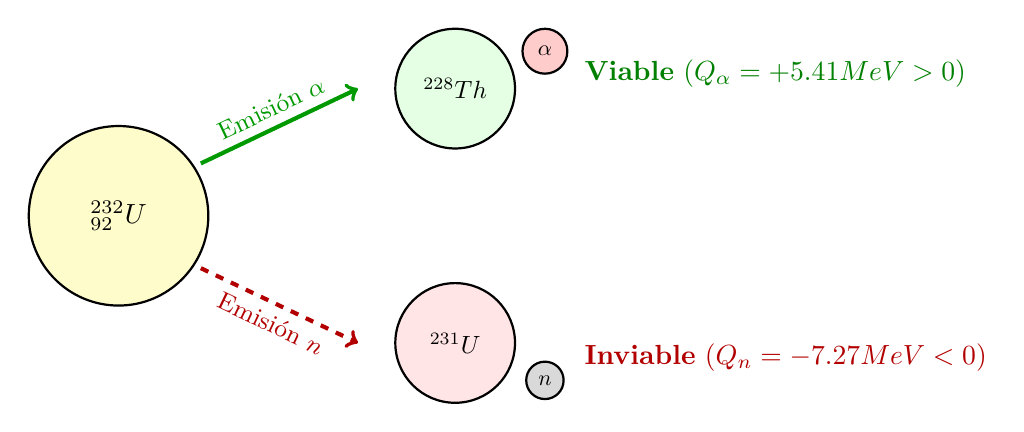
\begin{tikzpicture}[scale=0.95]
  % Núcleo Padre
  \draw[thick, fill=yellow!20] (0,0) circle (1.2) node[black] {${}_{92}^{232}\text{U}$};

  % Rama Alpha (Permitida)
  \draw[->, line width=1.5pt, green!60!black] (1.1,0.7) -- (3.2,1.7) node[midway, above, sloped] {\small Emisión $\alpha$};
  \draw[thick, fill=green!10] (4.5,1.7) circle (0.8) node[black, scale=0.9] {${}^{228}\text{Th}$};
  \draw[thick, fill=red!20] (5.7,2.2) circle (0.3) node[black, scale=0.8] {$\alpha$};
  \node[green!50!black, right] at (6.1,1.9) {\textbf{Viable} ($Q_\alpha = +5.41\text{ MeV} > 0$)};

  % Rama Neutrón (Prohibida)
  \draw[->, line width=1.5pt, red!70!black, dashed] (1.1,-0.7) -- (3.2,-1.7) node[midway, below, sloped] {\small Emisión $n$};
  \draw[thick, fill=red!10] (4.5,-1.7) circle (0.8) node[black, scale=0.9] {${}^{231}\text{U}$};
  \draw[thick, fill=gray!30] (5.7,-2.2) circle (0.25) node[black, scale=0.8] {$n$};
  \node[red!70!black, right] at (6.1,-1.9) {\textbf{Inviable} ($Q_n = -7.27\text{ MeV} < 0$)};
\end{tikzpicture}
\end{center}

\end{problema}